\documentclass{eecslides}
\mode<presentation>
% \usecolortheme{BBSDark}

%%------------------
% Language and font
\usepackage[english]{babel}
\usepackage[utf8]{inputenc}

%%------------------
\usepackage{graphicx}
\usepackage{color}
\usepackage{tikz}
\usetikzlibrary{calc, shapes, backgrounds, arrows}

% --- include packages
\usepackage{subfigure}
\usepackage{multicol}
\usepackage{amsthm}
\usepackage{mathrsfs}
\usepackage{amsmath}
\usepackage{amssymb}

%%------------------
\DeclareRobustCommand\refmark[1]{\textsuperscript{\ref{#1}}}

%%------------------ Tune the template
\setbeamertemplate{blocks}[rounded][shadow=false]
% \setbeamertemplate{title page}[default][colsep=-4bp,rounded=true]


%------------- Contenu de la page de titre -------------%

\title[Beamer template]{Beamer template demo}
\date{}
\author[KevCaz]{Kevin Cazelles}
\institute{Integrative Biology, University of Guelph}
\vspace{0.4cm}
\vspace{0.6cm}
\website{kevincazelles.fr}

%--------------------------%


%-----------------------------------------%
%------------- Tilte Page -------------%
%-----------------------------------------%


\begin{document}

\begin{frame}
  \titlepage
\end{frame}







%-----------------------------------------------%
%-------------      Section 1      -------------%
%-----------------------------------------------%

\section{Text}

%------------- Slide 1 -------------%

\begin{frame}
    \frametitle{Random text}
    \framesubtitle{Lorem ipsum}
        Lorem ipsum dolor sit amet, consectetur adipisicing elit, sed do eiusmod
        tempor incididunt ut labore et dolore magna aliqua. Ut enim ad minim
        veniam, quis nostrud exercitation ullamco laboris nisi ut aliquip ex
        ea commodo consequat.
\end{frame}


%------------- Slide 2 -------------%

\begin{frame}

  \frametitle{Tune the text size}

    \HUGE{HUGE},\\ \huge{huge}, \LARGE{LARGE},
    \large{large}, \normalsize{normalsize}, \small{small}, \footnotesize{footnotesize}, \scriptsize{scriptsize}, \tiny{tiny}, \Tiny{Tiny}, \TINY{Tiny}.


\end{frame}


%------------- Slide 3 -------------%

\begin{frame}

  \frametitle{Tune even more}

  Family:
  \rmfamily{rmfamily}, \sffamily{sffamily} or \ttfamily{ttfamily}.

  Shape:
  \upshape{upshape} \itshape{itshape} \slshape{slshape} \scshape{scshape}.

  Series:
  \bfseries{bfseries} \mdseries{mdseries}

\end{frame}


%------------- Slide 4 -------------%

\begin{frame}

  \frametitle{Maths}

  In line $\sum n$

  \begin{eqnarray}
    E(t) &=& 1 - cos(t) \\
    \dot{P}(t) &=& \left(-r_P + h_{EP}E(t) + \frac{1}{h_{PZ}}\frac{h_{PZ}P(t)}{h_{PZ}P(t)+h_{DZ}D(t)}\Phi \right)P(t)\\
    \dot{D}(t) &=& dP(t) -  \frac{1}{h_{PD}}\frac{h_{DZ}D(t)}{h_{PZ}P(t)+h_{DZ}D(t)}\Phi D(t)\\
    \dot{Z}(t) &=& \left(-r_Z+\Phi\right)Z(t)
  \end{eqnarray}

\end{frame}

%-----------------------------------------------%
%-------------      Section 2      -------------%
%-----------------------------------------------%

    \section{Figures and tables}

    %------------- Slide 5 -------------%
    \begin{frame}
        To improve the visual style of the presentation, use the color of this
        template in your figures:

        \begin{itemize}
          \item blue \#85b6d5
          \item red \#e080a3
          \item green \#d2e09c
          \item gris rgb(96,96,96) \#606060
        \end{itemize}

      \end{frame}


    %------------- Slide 6 -------------%
    \begin{frame}
        \frametitle{FIGURE}
            \begin{figure}
                \centering
                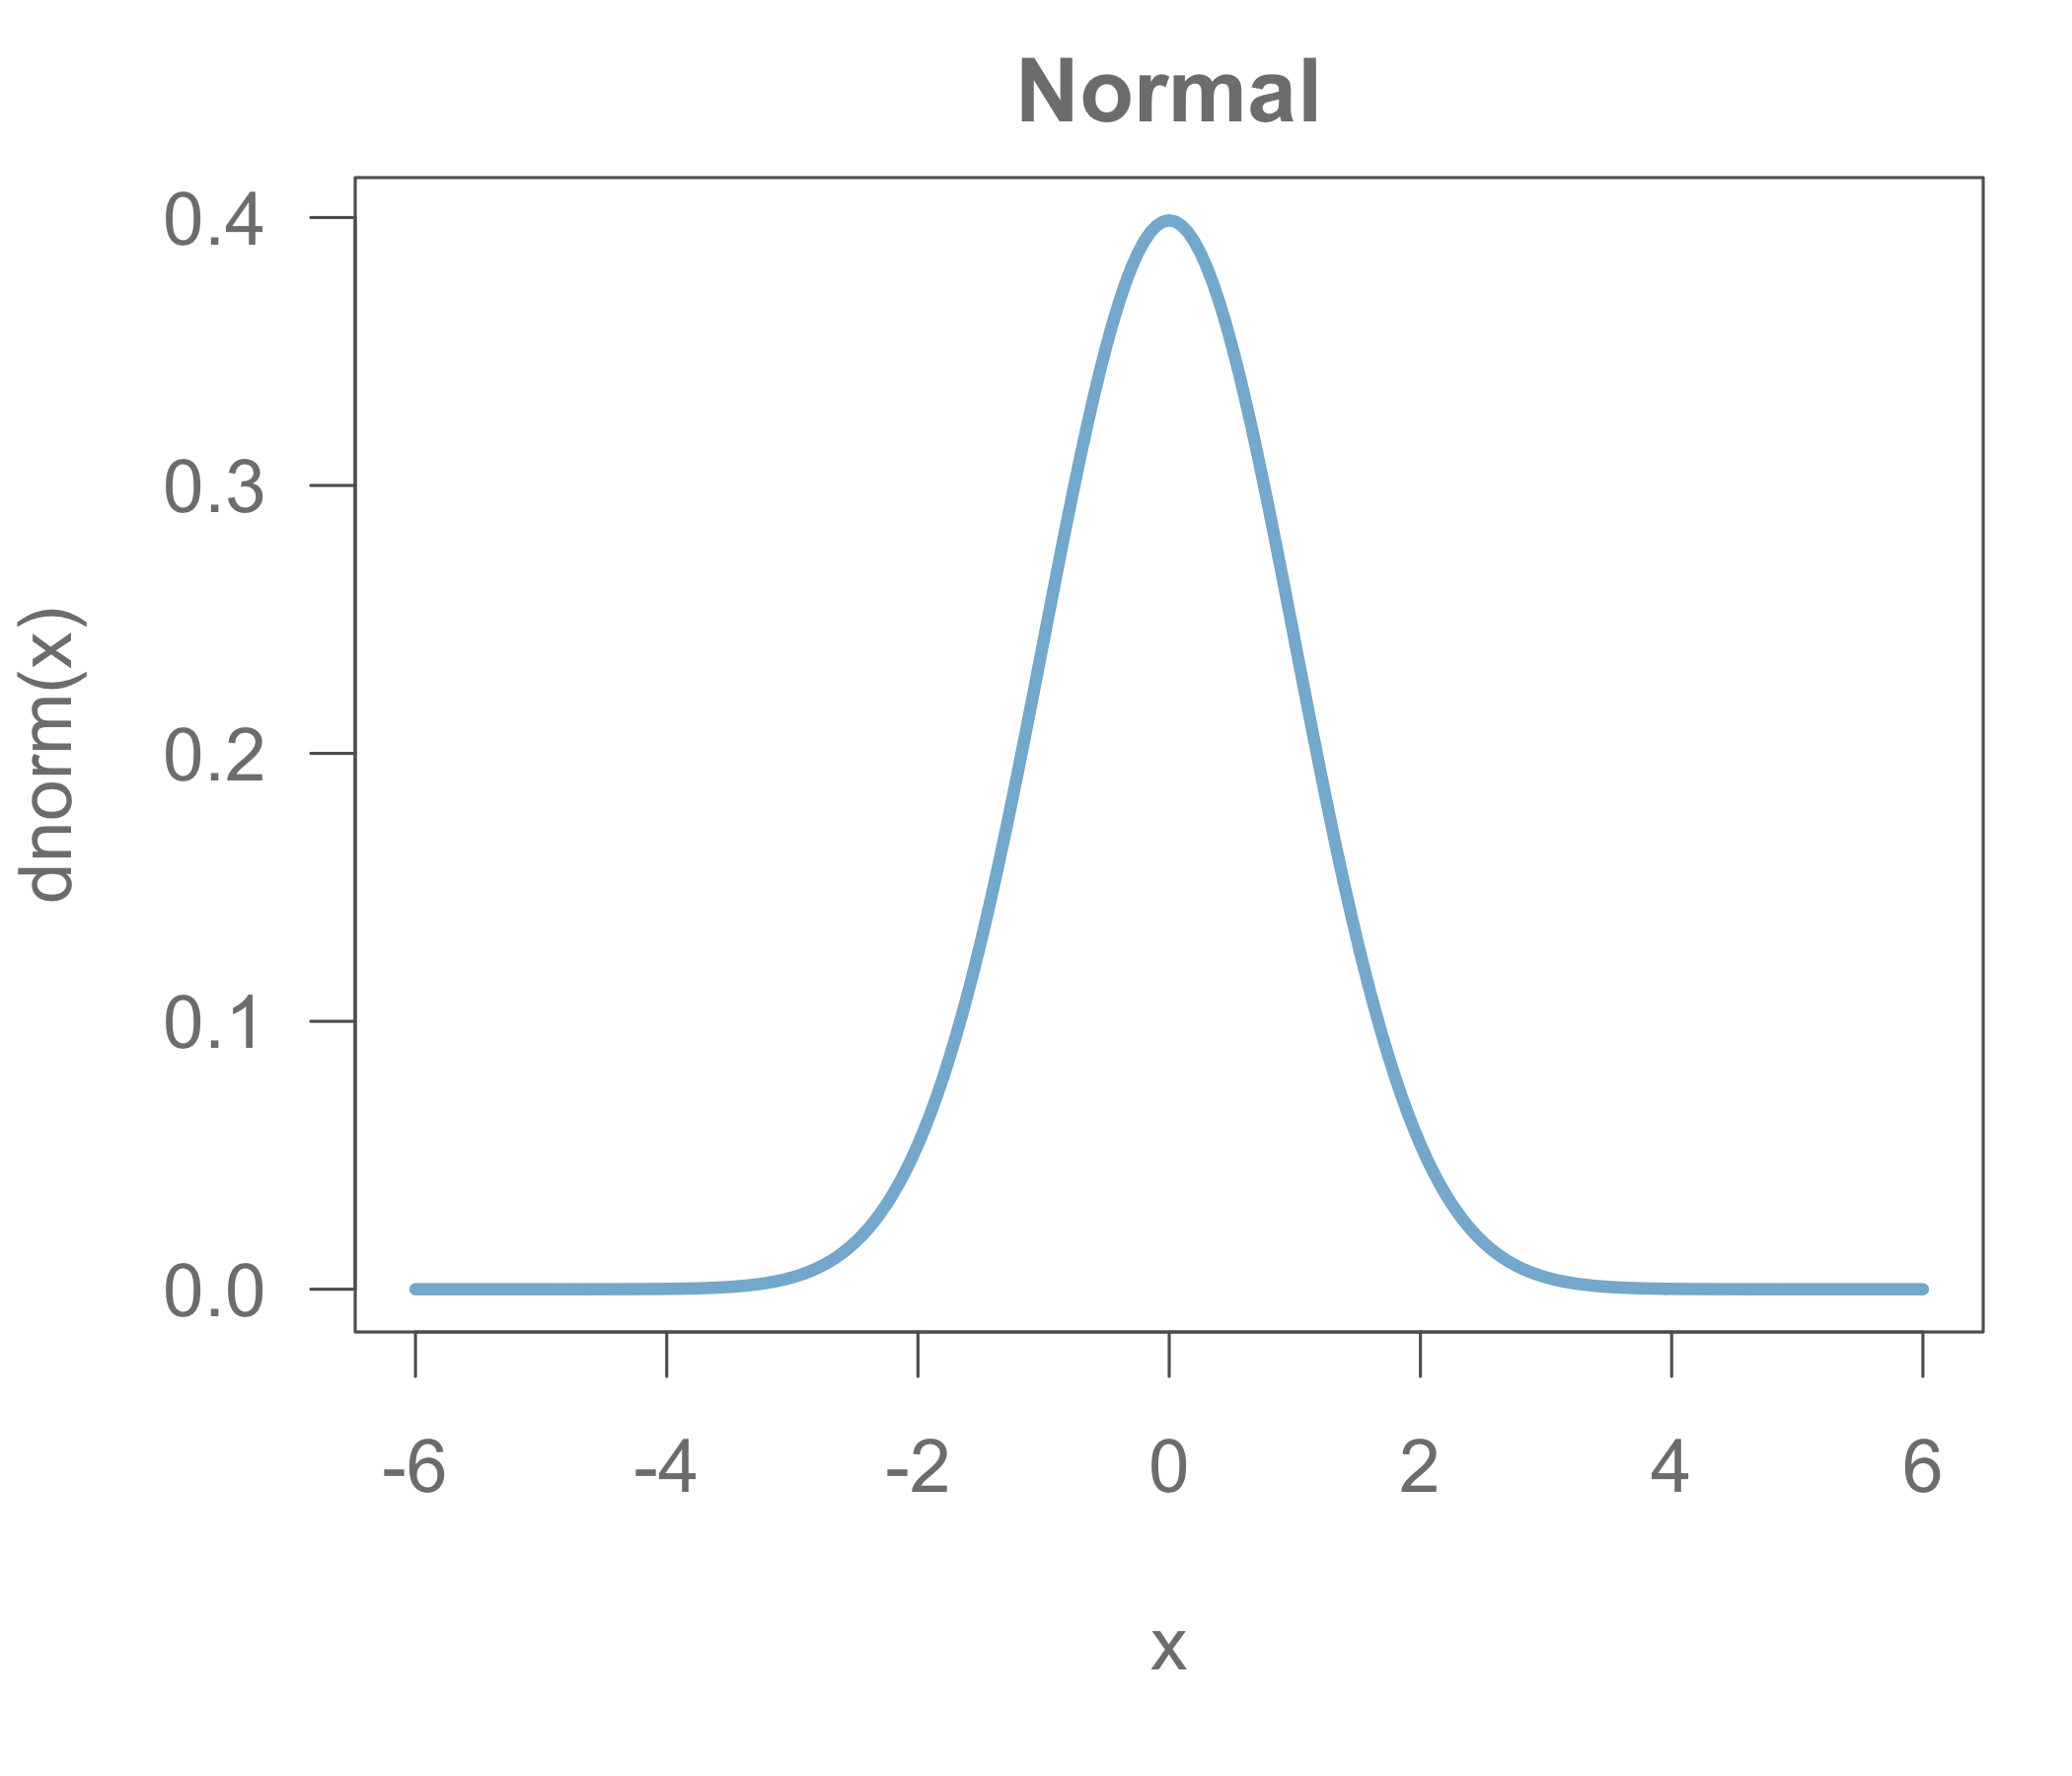
\includegraphics[width=.8\textwidth]{./fig/fig1.png}
                % 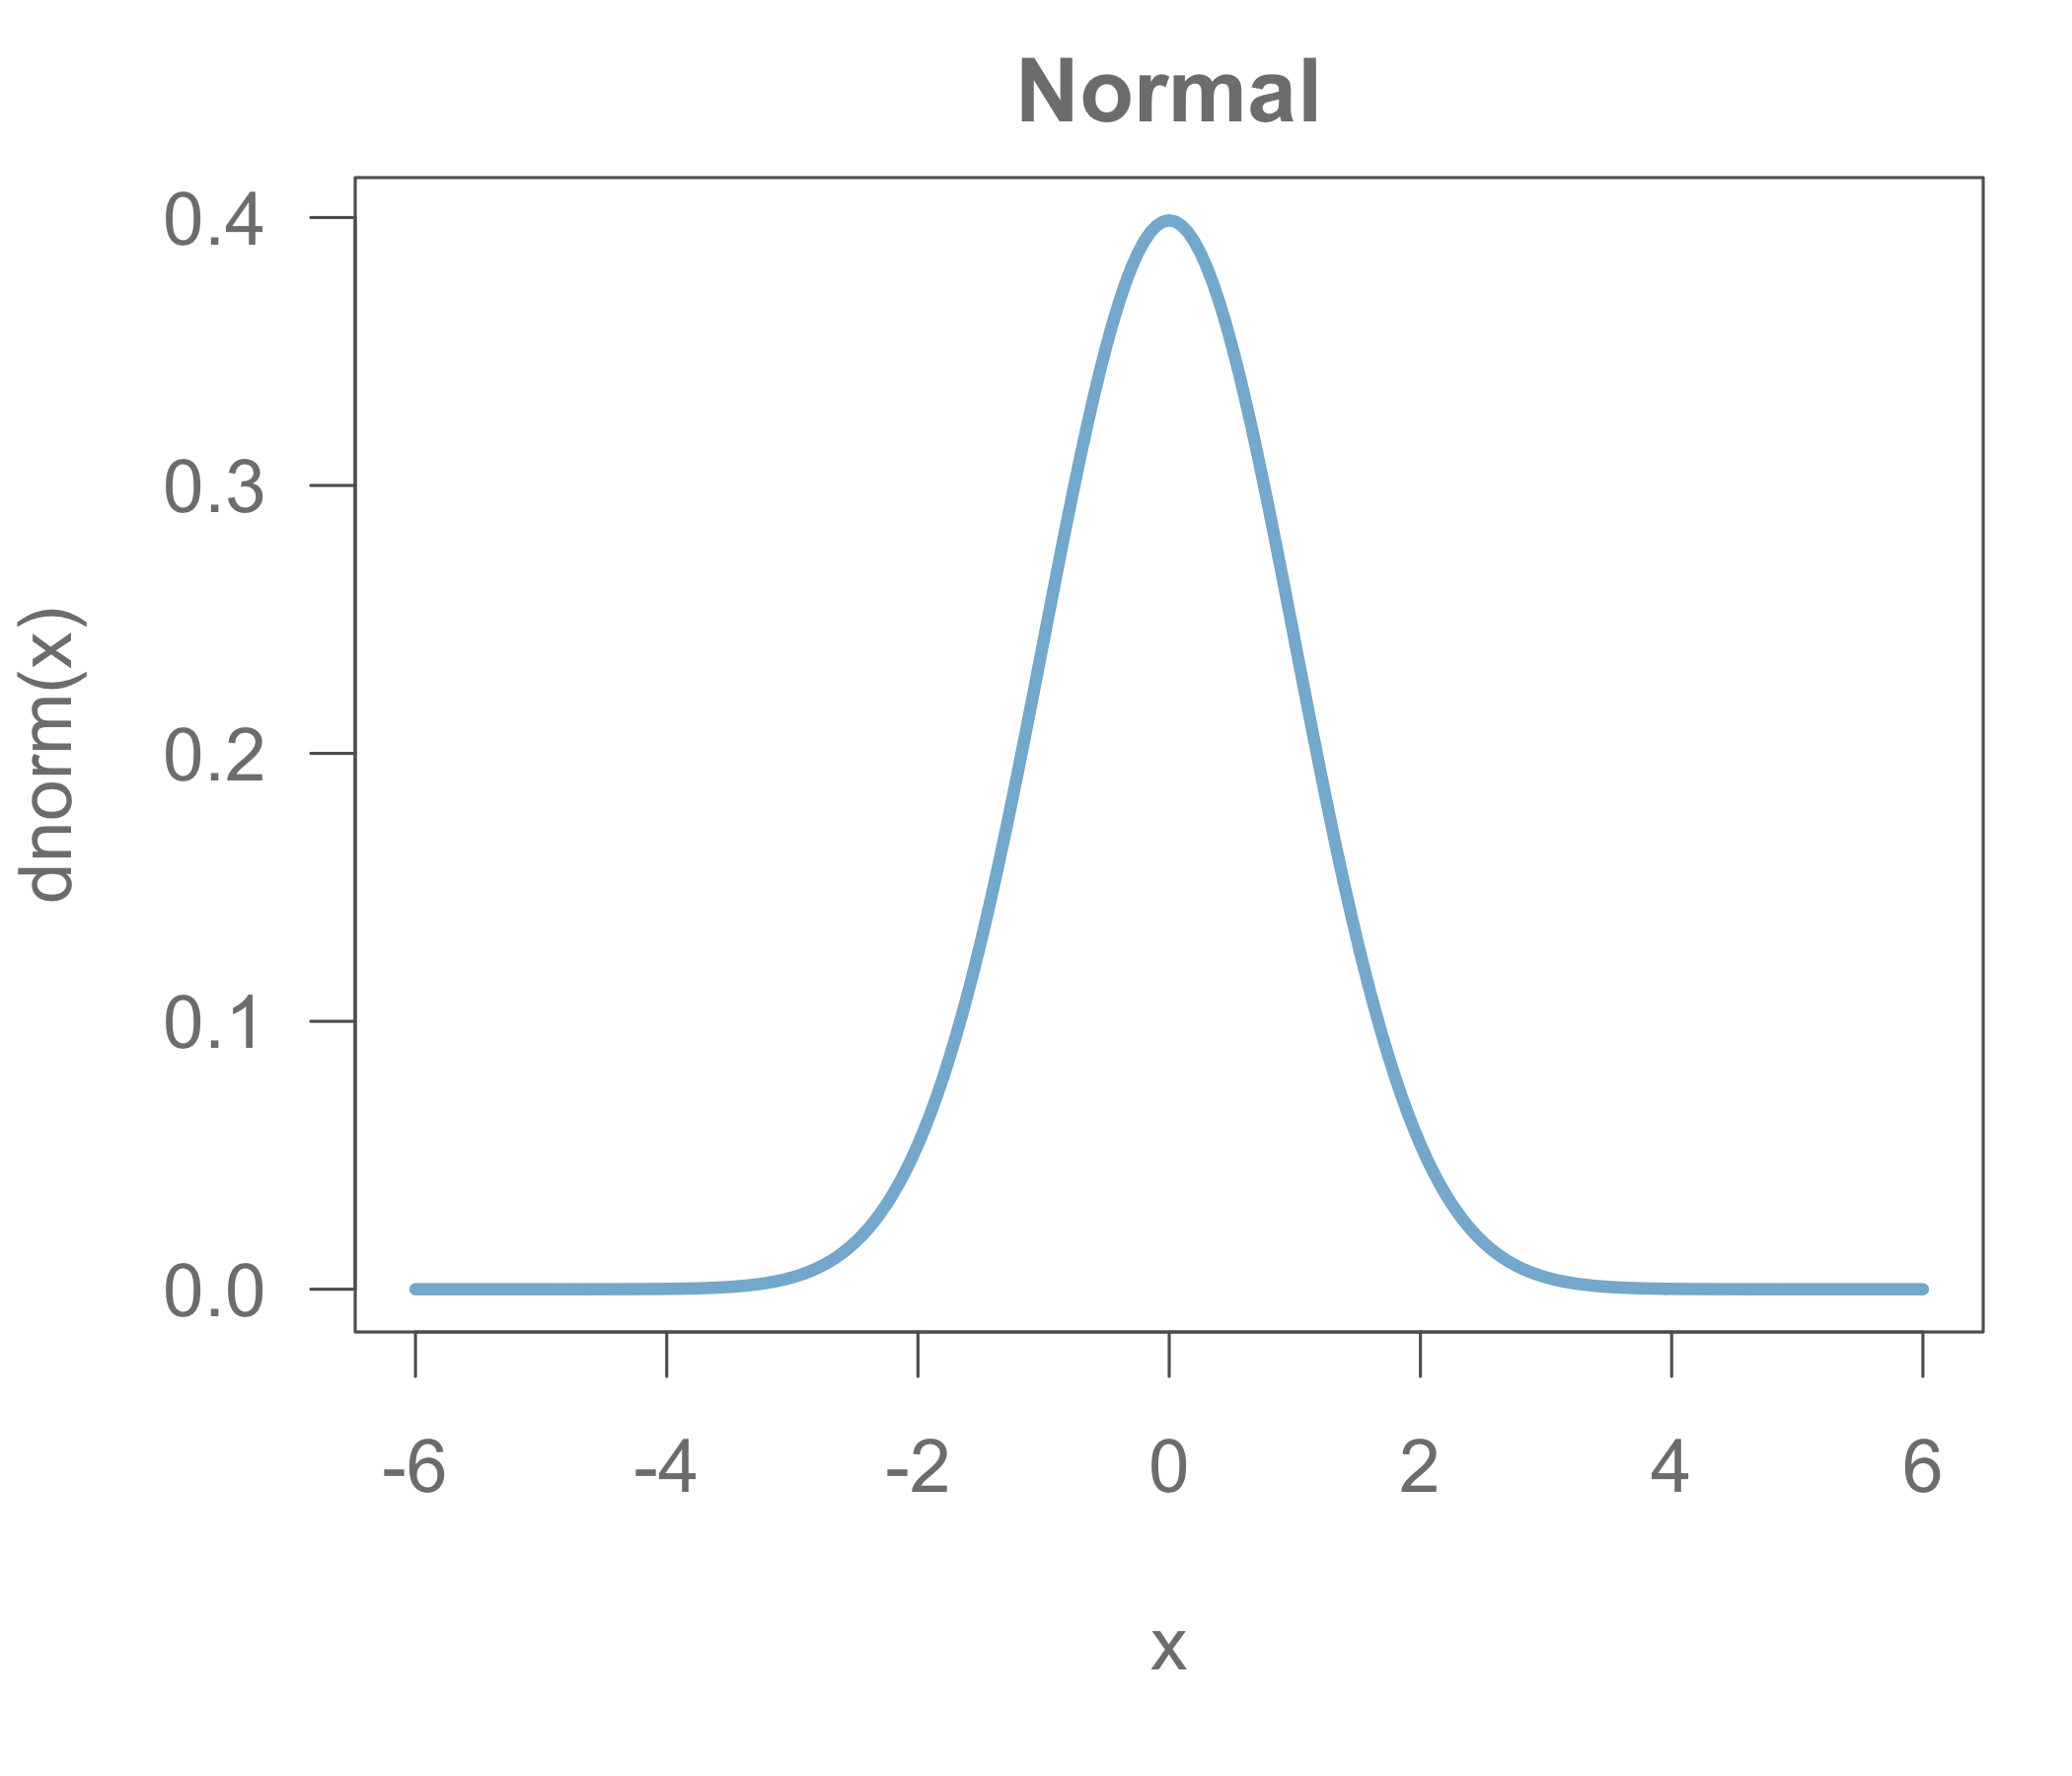
\includegraphics[scale=0.12]{./fig/fig1.png}
            \end{figure}
    \end{frame}


    %------------- Slide 7 -------------%
    \begin{frame}
        \frametitle{TABLE}

    \begin{table}
    \begin{tabular}{|l|l|l|l|l|l|}
      Community states & B & C & D & E & TTIB-compatible \\ \hline
      \(S_{0}\) & 0 & 0 & 0 & 0 & yes \\
      \(S_{1}\) & 0 & 0 & 0 & 1 & no \\
      \(S_{2}\) & 0 & 0 & 1 & 0 & yes \\
      \(S_{3}\) & 0 & 0 & 1 & 1 & yes \\
      \(S_{4}\) & 0 & 1 & 0 & 0 & yes \\
      \(S_{5}\) & 0 & 1 & 0 & 1 & yes \\
      \(S_{6}\) & 0 & 1 & 1 & 0 & yes \\
      \(S_{7}\) & 0 & 1 & 1 & 1 & no
    \end{tabular}
  \end{table}

  \end{frame}


%-----------------------------------------------%
%-------------      Section 3      -------------%
%-----------------------------------------------%


    %------------- Slide 2 -------------%
    \begin{frame}
      \frametitle{BLOCKS}

      \begin{block}{RegBlock}
          A regular block
      \end{block}

      \begin{exampleblock}{ExBlock}
          An example block
      \end{exampleblock}

      \begin{alertblock}{AlertBlock}
        Pass auf!
      \end{alertblock}


    \end{frame}


    %------------- Perspective D2 -------------%
    \begin{frame}
        \frametitle{Numbered list + pause + alert}

        \begin{large}
        \begin{enumerate}
            \item \textbf{First item} \alert<4>{to be highlighted},
            \pause
            \item \textbf{Second item} \alert<4>{to be highlighted},
            \pause
            \item \textbf{Third item} list's end,
        \end{enumerate}
      \end{large}

        \pause
        \LARGE{ALERT} (see above)

    \end{frame}
    %--------------------------%




    %---------------------------------------------------%
    %------------- Section 4 : Perspectives -------------%
    %---------------------------------------------------%


    \section{Advanced features}


      %-------------  tikzpicture -------------%
        \begin{frame}

          \frametitle{Use tikzpicture!}

          % Found here http://www.texample.net/tikz/examples/coin-flipping/

          \tikzset{
            head/.style = {fill = bssred!90!bssblue,
                           label = center:\textsf{\Large H}},
            tail/.style = {fill = bssblue, text = black,
                           label = center:\textsf{\Large T}}
          }
          \begin{tikzpicture}[
              scale = 1.2, transform shape, thick,
              every node/.style = {draw, circle, minimum size = 10mm},
              grow = down,  % alignment of characters
              level 1/.style = {sibling distance=3cm},
              level 2/.style = {sibling distance=4cm},
              level 3/.style = {sibling distance=2cm},
              level distance = 1.25cm
            ]
            \node[fill = gray!10, shape = rectangle, rounded corners,
              minimum width = 6cm, font = \sffamily] {Coin flipping}
            child { node[shape = circle split, draw, line width = 1pt,
                    minimum size = 10mm, inner sep = 0mm, font = \sffamily\large,
                    rotate=30] (Start)
                    { \rotatebox{-30}{H} \nodepart{lower} \rotatebox{-30}{T}}
             child {   node [head] (A) {}
               child { node [head] (B) {}}
               child { node [tail] (C) {}}
             }
             child {   node [tail] (D) {}
               child { node [head] (E) {}}
               child { node [tail] (F) {}}
             }
            };

            % Filling the root (Start)
            \begin{scope}[on background layer, rotate=30]
              \fill[head] (Start.base) ([xshift = 0mm]Start.east) arc (0:180:5mm)
                -- cycle;
              \fill[tail] (Start.base) ([xshift = 0pt]Start.west) arc (180:360:5mm)
                -- cycle;
            \end{scope}

            % Labels
            \begin{scope}[nodes = {draw = none}]
              \path (Start) -- (A) node [near start, left]  {$0.5$};
              \path (A)     -- (B) node [near start, left]  {$0.5$};
              \path (A)     -- (C) node [near start, right] {$0.5$};
              \path (Start) -- (D) node [near start, right] {$0.5$};
              \path (D)     -- (E) node [near start, left]  {$0.5$};
              \path (D)     -- (F) node [near start, right] {$0.5$};
              \begin{scope}[nodes = {below = 11pt}]
                \node [name = X] at (B) {$0.25$};
                \node            at (C) {$0.25$};
                \node [name = Y] at (E) {$0.25$};
                \node            at (F) {$0.25$};
              \end{scope}
              \draw[densely dashed, rounded corners, thin]
                (X.south west) rectangle (Y.north east);
            \end{scope}
          \end{tikzpicture}

        \end{frame}
      %--------------------------%




\end{document}
